\documentclass[a4paper,
               %boxit,
               %titlepage,   % separate title page
               %refpage      % separate references
              ]{jacow}
%
% CHANGE SEQUENCE OF GRAPHICS EXTENSION TO BE EMBEDDED
% ----------------------------------------------------
% test for XeTeX where the sequence is by default eps-> pdf, jpg, png, pdf, ...
%    and the JACoW template provides JACpic2v3.eps and JACpic2v3.jpg which
%    might generates errors, therefore PNG and JPG first
%
\makeatletter%
	\ifboolexpr{bool{xetex}}
	 {\renewcommand{\Gin@extensions}{.pdf,%
	                    .png,.jpg,.bmp,.pict,.tif,.psd,.mac,.sga,.tga,.gif,%
	                    .eps,.ps,%
	                    }}{}
\makeatother

% CHECK FOR XeTeX/LuaTeX BEFORE DEFINING AN INPUT ENCODING
% --------------------------------------------------------
%   utf8  is default for XeTeX/LuaTeX
%   utf8  in LaTeX only realises a small portion of codes
%
\ifboolexpr{bool{xetex} or bool{luatex}} % test for XeTeX/LuaTeX
 {}                                      % input encoding is utf8 by default
 {\usepackage[utf8]{inputenc}}           % switch to utf8

\usepackage[USenglish]{babel}

\usepackage[final]{pdfpages}
\usepackage{multirow}
\usepackage{ragged2e}
\usepackage{todonotes}
\usepackage{epstopdf}

%
% if BibLaTeX is used
%
\ifboolexpr{bool{jacowbiblatex}}%
 {%
  \addbibresource{jacow-test.bib}
  \addbibresource{biblatex-examples.bib}
 }{}
\listfiles

%
% command for typesetting a \section like word
%
\newcommand\SEC[1]{\textbf{\uppercase{#1}}}

%%
%%   Lengths for the spaces in the title
%%   \setlength\titleblockstartskip{..}  %before title, default 3pt
%%   \setlength\titleblockmiddleskip{..} %between title + author, default 1em
%%   \setlength\titleblockendskip{..}    %afterauthor, default 1em

%\copyrightspace %default 1cm. arbitrary size with e.g. \copyrightspace[2cm]

% testing to fill the copyright space
%\usepackage{eso-pic}
%\AddToShipoutPictureFG*{\AtTextLowerLeft{\textcolor{red}{COPYRIGHTSPACE}}}

\begin{document}

\title{openMMC: An Open Source Modular Firmware for Board Management}

\author{H. A. Silva\thanks{henrique.silva@lnls.br}, G. B. M. Bruno, LNLS, Campinas, Brazil}

\maketitle

%
\begin{abstract}
  openMMC is an open source firmware designed for board management in MicroTCA systems.
  It has a modular architecture providing decoupling between application,
  board and microcontroller-specific routines, making it useful as a base for many
  different designs, even those using less powerful controllers.
  Despite being developed in a MicroTCA context, the firmware can be easily adapted
  to other hardware platforms and communication protocols.
  The firmware is based on the FreeRTOS operating system, over which each monitoring function
  (sensors, LEDs, Payload management, etc) runs its own independent task.
  The OS, despite its reduced footprint, also provides numerous tools for reliable
  communication among the tasks, controlling the board efficiently.
\end{abstract}

\section{Introduction}

LNLS Beam Diagnostics team is currently developing the Sirius' Beam Position Monitor (BPM) electronics and has adopted the MicroTCA.4\textregistered~ standard by PICMG \cite{picmg-mtca} in its boards designs \cite{bpm-electronic-spec}.

The main board on the electron BPM system is the AMC FMC Carrier (AFC) \cite{afc-ohwr}, which is a general purpose FPGA board that hosts up to two mezzanine cards in FMC form factor.
Those smaller cards carried by AFC can be implemented to have many different applications (e.g. fast digitizers, SFP modules, data pre-processing modules, RS485 communication). In the BPM application, fast digitizer FMCs will be used in order to read the BPM analog signals.

AMC boards, as the application boards are called in the MicroTCA system, must have implemented a Module Management Controller (MMC), which usually is a microcontroller responsible for monitoring the board health and acting as a communication channel between the system manager and application using Intelligent Platform Management Interface (IPMI) \cite{ipmi}.

openMMC was created to be an open source (using GPLv3 license) modular and generic firmware, easily portable to other platforms. It runs over FreeRTOS, which gives the developer a wide set of tools to implement complex monitoring functions or advanced hardware control.
Given its modular independent structure, it is possible to use the firmware in applications outside MicroTCA environment with little effort, changing the communication protocol in its lower layers, for example.

The project development is being versioned in a GitHub repository \cite{openmmc-github}, using pull requests and issues tracking as its main collaboration tools.

\section{Motivation}
The development of openMMC started after some unfruitful tests with the available open source MMC implementations.
Those firmwares were developed to run on specific target boards, requiring a substantial effort in order to port them to AFC's hardware and begin a functional evaluation process.

After some attempts, it was clear that porting the code basically meant to rewrite it from scratch, given that its low level driver and application functions were deeply intertwined.

The hardware flexibility offered by MicroTCA was not being accompained by its MMC firmware architecture, since each board implementation had to recreate the managing firmware. openMMC was thought to be the hardware independent firmware that could meet this need.

\section{FreeRTOS}
FreeRTOS \cite{freertos} is a popular open source real time operating system for embedded controllers that has already been ported to a wide range of CPU architectures.

It features a preemptive scheduler that allows the application code to run multiple tasks in parallel with a single core.
The scheduler decides which task will run based on its priority. More important tasks are always executed first, whilst blocking the lower priority ones.
If one or more tasks are on the same priority level, a round-robin time slice method is applied, ensuring that all of them are executed within its time limits.

Most of OS-native tools used in communication between tasks are also implemented on FreeRTOS (e.g. semaphores, software timers, queues).
The developer can also use some unique functions provided, such as direct-to-task notifications, event groups and co-routines.

Except for task creation, all tools on FreeRTOS can be stripped from its compilation, reducing resource usage, thus enabling use of cheaper and lower-power microcontrollers.

FreeRTOS project uses a modified GPLv3 license, which allows the user to implement its application on top of the OS without having to publish proprietary code \cite{freertos-license}.

\section{Firmware Structure}
The firmware was structured in order to be easy to upgrade and port to different boards and controllers.
Therefore four different abstraction layers are implemented: \emph{Application}, \emph{Hardware Abstraction}, \emph{Port} and \emph{Driver}, arranged as in Figure \ref{fig:fw-structure}.

\begin{figure}[!htb]
\centering
%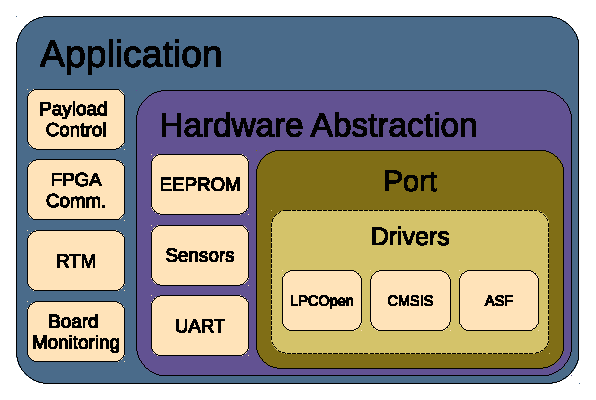
\includegraphics[scale=0.8]{fw-structure.eps}
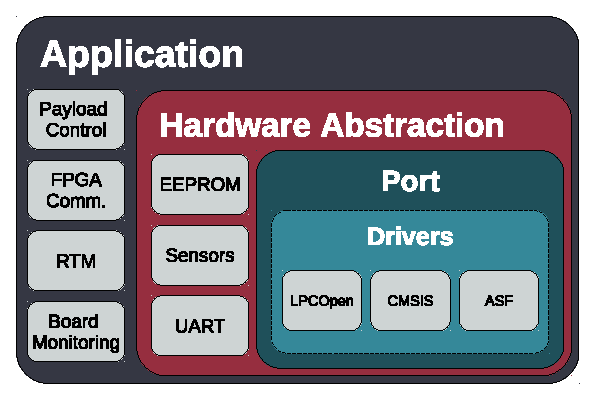
\includegraphics[scale=0.8]{fw-structure-dark.eps}
\caption{openMMC firmware structure}
\label{fig:fw-structure}
\end{figure}

\subsection{Application}
The Application layer holds high-level tasks responsible for deciding which action will be taken based on the information provided by the lower level layers. Most of the functions implemented on this level are state-machine based, regurlarly checking and actuating on the board status.

\subsection{Hardware Abstraction}
In the Hardware Abstraction Layer (HAL) lies all the functions that interfaces with the board peripheral hardware, making the internal calls to the IC registers transparent to the caller for example. Since any board can benefit from a module in this layer, they are all stored together inside "modules" folder.

An exception in the HAL is the IPMI Protocol module, that does not target any specific peripheral hardware. Instead, it is responsible to manage IPMI protocol messages internally, decoding packets, asserting checksums and building responses accordingly.

The following modules were already implemented and tested in LNLS' AFC board:
\begin{Itemize}

\item IPMI Protocol
\item Watchdog Timer
\item SCANSTA111 JTAG Switch
\item ADN4604 Clock Crossbar Switch
\item AD84XX DAC
\item AT24MAC EEPROM
\item 24xx64 EEPROM
\item Hotswap Handle
\item LM75 Temperature Sensor
\item MAX6642 Temperature Sensor
\item INA220 Voltage and Current Sensor
\item HPM Upgrade
\item PCA9554 I/O Expander
\item Si57X Oscillator
\item UART Debug interface

\end{Itemize}

\subsection{Port}
The Port layer serves as a connection between \emph{Driver} and the upper layers.
Its purpose is to mask all functions provided by the controller drivers so that the upper layers only call generic functions defined in this level, as demonstrated in Figure \ref{fig:port-example}.

\begin{figure}[!htb]
\centering
%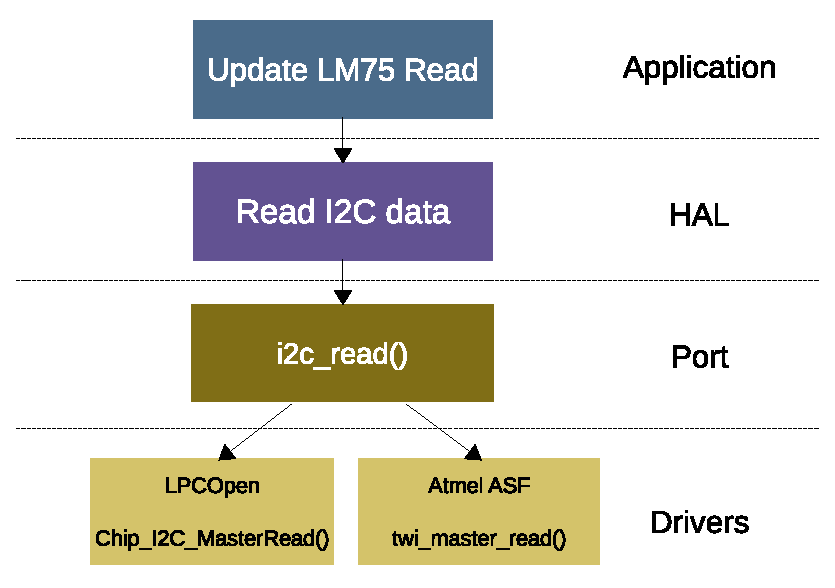
\includegraphics[scale=0.6]{port-example.eps}
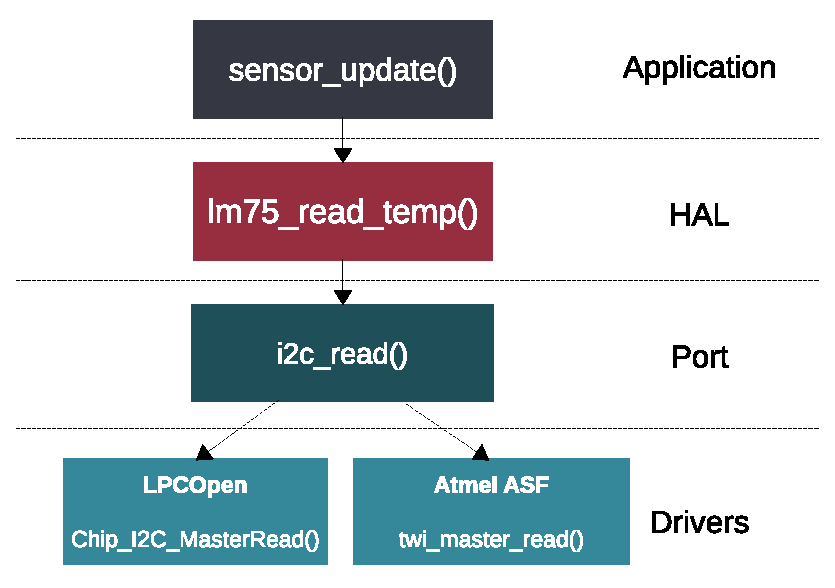
\includegraphics[scale=0.6]{port-example-dark.eps}
\caption{openMMC sensor update function call sequence}
\label{fig:port-example}
\end{figure}

This layer presents a few restrictions regarding its structure. Developers in charge of implementing new hardware drivers must follow the port layer functions' signature in order to maintain compatibility throughout the firmware.

Currently, there is only one port maintaned in mainline openMMC, which targets LPC17 family chips.
Development of a port to ATxMega128 CPU has been initiated by GSI \cite{gsi-mmc}.

\subsection{Drivers}
The lowest layer is where the microcontroller peripheral drivers are implemented, accessing directly the hardware to control the outputs.

\section{Bootloader}
Having a small footprint makes it possible to store more than one image of the running firmware, easing the system's upgrade process. Taking advantage of this property, a Bootloader scheme was developed in order to manage the controller's memory sections and reserve a portion of the ROM to store an updated firmware. An example of the internal memory divison in a LPC1764 controller can be seen in Figure \ref{fig:bootloader-mem}.

\begin{figure}[!htb]
\centering
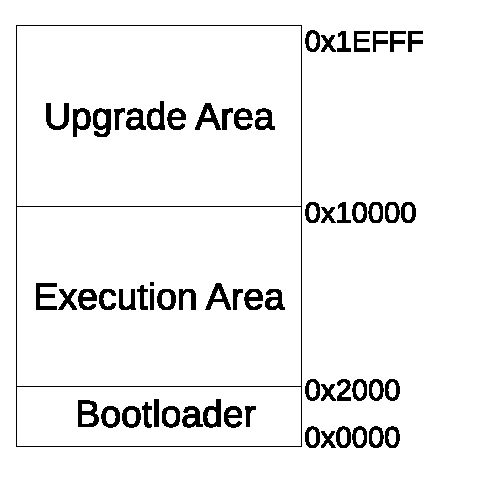
\includegraphics[scale=0.6]{bootloader-mem.eps}
\caption{LPC1764 ROM organization with openMMC}
\label{fig:bootloader-mem}
\end{figure}


The new firmware is sent to the MMC broken in small packages using HPM update protocol \cite{hpm}, defined by PICMG.
The controller then writes page by page the new firmware in the reserved ROM section and also adds a update flag to the bootlader, indicating that this firmware is the more recent version and should be moved to the proper section in order to be executed.

The bootlader is always executed first in power-up sequence, checking whether there is a new firmware to write into execution section. If not, it just moves the program execution flow to the starting point of the user code area.

\section{Build Automation}
CMake is a software designed to automate build systems \cite{cmake}, widely used in projects where the compilation chain has more than one build target and needs to manipulate multiple sources. It implements its own scripting language that allows the user to fully customize each build without having to worry about sources dependencies.

Using this tool with openMMC allows developers to fit the firmware to the board hardware just by adding new modules in the compilation list present on each board port folder.
The user is also able to set new compilation flags or link new libraries almost effortless.

\section{Board Porting}
openMMC also allows the user to easily port the firmware to a different board with other peripheral hardware configuration while keeping the target controller.

Since all peripheral hardware drivers are implemented as modules in the \emph{Hardware Abstraction Layer}, only the \texttt{CMakeLists.txt} file inside the board folder have to be changed. In this file, all modules needed in each hardware configuration are selected based on a list parameter. When CMake is called to generate the automatic Makefiles, it parses this argument and includes all selected modules sources and dependecies in the compilation chain.

\section{Code Size}
openMMC has a small memory footprint, which makes it perfect for embedded environments that traditionally have limited resources.
Table \ref{table:mem_usage} presents openMMC's average RAM usage and code size in ROM after compiling in both minimal and standard configurations for AFC BPM board, using GCC's optimization flag -Os.

\begin{table}[hbt]
  \centering
  \caption{openMMC resources usage}
  \label{table:mem_usage}
  \begin{tabular}{lcc}
    \toprule
    \textbf{Configuration} & \textbf{RAM [kB]} & \textbf{ROM [kB]} \\
    \midrule
    Minimal                & 5.54               & 20.91  \\
    Standard               & 8.07               & 29.69  \\
       \bottomrule
  \end{tabular}
\end{table}

\section{Continuous Integration}
Every modification in the application layer must be tested across all boards and controllers ports to assert that the firmware remains compatible.

Confirming that the firmware compiles with every variant option becomes very difficult as the ports count increases.
Using a Continuous Integration tool allows the maintainer to run dedicated tests after each commit on the main repository and automatically reports if the lattest change has made any port unusable.
Travis C.I. \cite{travis-ci} uses a simple script written in its own language to install the needed toolchains and by tracking the latest commits on the repository branches, it is able to perform build tests on them, ensuring that the latest modification is compatible with all board and controller ports.

\section{Documentation}
The firmware documentation is written using Doxygen style \cite{doxygen}. This way, the documentation format is completely automated and can have many different output formats such as HTML, \LaTeX , XML, RTF, etc.

By hosting the firmware code in GitHub repository, one is able to use a feature called GitHub Pages, in which a small website for generic use can be hosted simply by adding a new branch named \emph{gh-pages} in the main repository. openMMC documentation has been uploaded to GitHub pages, but it is still under development \cite{openmmc-gh-page}.

Using this tool simplifies code documentation update, since it just needs to be regenerated by Doxygen after each change and pulled to its respective GitHub Pages branch.

\section{Acknowlegments}
The authors would like to thank K. Macias from Creotech Instruments SA for the extensive firmware debug and P. Miedzik from GSI for the initial discussions in the firmware structure definition and by suggesting FreeRTOS as a base for the project.

\iffalse  % only for "biblatex"
	\newpage
	\printbibliography

% "biblatex" is not used, go the "manual" way
\else

\begin{thebibliography}{99}   % Use for  10-99  references
%\begin{thebibliography}{9} % Use for 1-9 references

\bibitem{picmg-mtca}
  PICMG MicroTCA Specification,
  \url{https://www.picmg.org/openstandards/microtca}

\bibitem{bpm-electronic-spec}
  D. O. Tavares et al.,
  ``Development of an Open-Source Hardware Platform for Sirius BPM and Orbit Feedback'',
  ICALEPCS'13, San Francisco, October 2013, p. 1039 (2013)

\bibitem{afc-ohwr}
  AMC FMC Carrier Project,
  \url{http://www.ohwr.org/projects/afc}

\bibitem{ipmi}
  Inteligent Platform Management Interface,
  \url{http://www.intel.com/content/www/us/en/servers/ipmi/ipmi-home.html}

\bibitem{openmmc-github}
  openMMC GitHub Repository,
  \url{https://github.com/lnls-dig/openMMC/}

\bibitem{freertos}
  FreeRTOS Project Page,
  \url{http://www.freertos.org/}

\bibitem{freertos-license}
  FreeRTOS modified GPLv3 license,
  \url{http://www.freertos.org/license.txt}

\bibitem{gsi-mmc}
  GSI MMC implementation repository,
  \url{https://github.com/qermit/JAMMCI/}

\bibitem{hpm}
  Hardware Platform Management Overview,
  \url{https://www.picmg.org/openstandards/hardware-platform-management/}

\bibitem{cmake}
  CMake Project,
  \url{https://cmake.org/}

\bibitem{travis-ci}
  Travis Countinous Integration tool,
  \url{https://travis-ci.org/}

\bibitem{doxygen}
  Doxygen Project,
  \url{http://www.stack.nl/~dimitri/doxygen/}

\bibitem{openmmc-gh-page}
  openMMC Documentation at GitHub Pages,
  \url{http://lnls-dig.github.io/openMMC/}



\end{thebibliography}

\fi

\end{document}
